
% Research question here? 
% Going to be challenging to have this not come across as a software design
% spec.. Let's try to get this section over with as little text wasted as
% possible... I feel silly writing these sections, since I ALWAYS skip over
% them when I'm reading other people's papers...
\projectname{} is our realization of correspondence checking and \simulator{}
as a useful platform to troubleshoot SDN controllers. In this section we discuss
our goals in designing \simulator{}, and the challenges we encountered in the process
of realizing these goals.

\subsection{Design Goals}

We seek to build a system that facilitates the process of troubleshooting.
First and foremost, we hope that \projectname{} can reproduce difficult bugs
observed in production networks, and automate the process of diagnosing their
causes. We also envision \projectname{} being used as a common repository for difficult, corner-case
scenarios known to have caused problems for other control platforms in the past.
Given these potential use cases, we require the design of the system to be
driven by the following requirements:

% Don't mention 'realism', since a simulation-based system just isn't real
% enough.

\noindent{\bf Comprehensive Failure Modes.} \projectname{} is primarily
focused on corner-case scenarios, which are the most difficult to anticipate
and cover for with traditional testing techniques. \projectname{} should
therefore support a wide range of failure modes at all components in the
system.

\noindent{\bf Realistic Networks.} We focus on large, production SDN
deployments. As today's datacenters may contain up to 100,000 hosts and 10,000
switches, our simulation infrastructure must be able to support large numbers
of switches. Note that we do not require the simulator to support efficient dataplane
forwarding however, as we focus on proactive control applications.

\noindent{\bf Wide range of usage scenarios.} The machinery in \simulator{}
is sophisticated enough to be applicable to a wide range of usage-patterns. We
hope to support automated use, yet perform well enough to support interactive
use For interactive use, the system must be able to deterministically replay
event sequences to allow user to explore their intuitions freely. % wat

\noindent{\bf Controller Agnostic.} The adoption of the system increases
dramatically if the control software under test does not need to be modified.
We aim to provide a framework that can run any SDN control stack, and model a
wide range of deployment scenarios.

\subsection{Components}

As depicted in Figure \ref{fig:system}, \projectname{} combines several
components to facilitate the process of troubleshooting SDN platforms:
\projectname{} takes input
from production traces, interactive manipulation, and synthetic trace
generation, and fuzzes these inputs to ensure that fixes are sufficiently general;
\projectname{}'s simulator supports large, sophisticated networks;
\projectname{} provides a deterministic, code-agnostic execution environment 
for running SDN control software; and provides efficient algorithms for
checking correspondence throughout the system execution. We now provide an
overview of each of these components, and the challenges we encountered in
realizing our goals.

\begin{figure*}[!t]
  \centering
  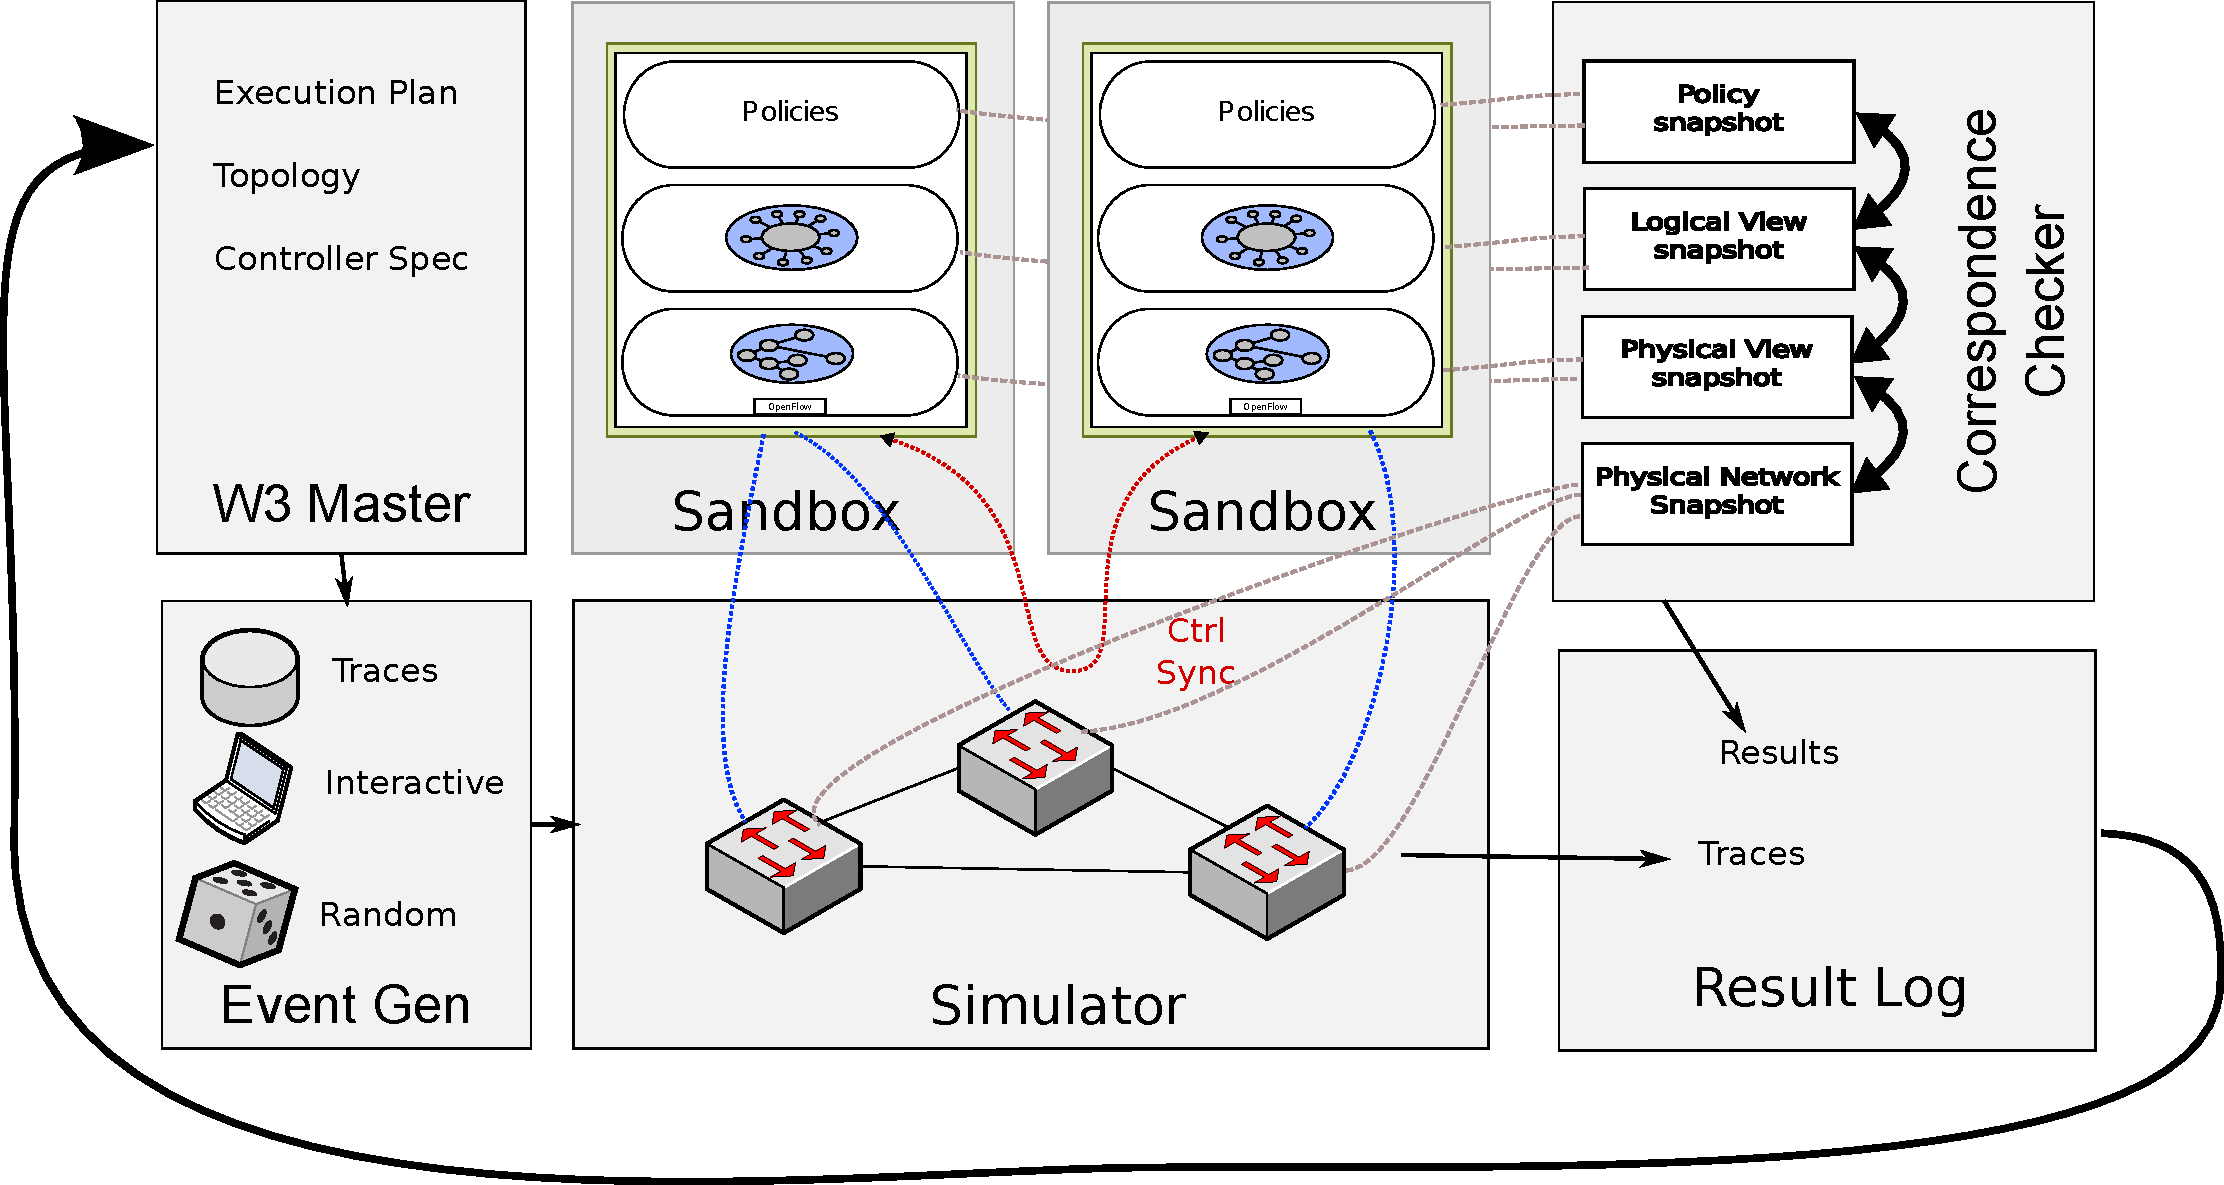
\includegraphics[width=0.8\textwidth]{../diagrams/architecture/architecture.pdf}
  \caption{System architecture}
  \label{fig:system}
\end{figure*}

\noindent{\bf Trace Input And Fuzzing.} Since a major goal \projectname{} was
to support a wide range of usage scenarios, % WAT does that even mean
we provide support for three different methods for generating network trace
inputs. The most common method is to insert failure and topology change logs
from production deployments into the simulator for replay. Input traces may
also be produced synthetically with configurable, random probabilities for
network events. Lastly, we support interactive use, where the troubleshooter
has complete control over network events, and is thereby free to explore her
intuitions in order to reproduce a failure mode she has in mind.

\noindent{\bf Simulator.} We have built a simulator for SDN networks,
where network devices and hosts are modeled as lightweight python objects. Within a single thread, we
are able to deterministically model the execution of very large networks.
Our simulated model supports a wide
range of failure modes, and provides fine-grained control over event
orderings, component failures, and other aspects of the system execution. Our
simulator currently supports switch failures, link failures, arbitrary packet
re-orderings, drops and delays, a fully general control plane.

The main challenge we encountered in the design of the simulator was the
maintaining large numbers of TCP connections to the
controller(s). Although the controllers themselves may be spread
over multiple physical servers, the main simulator must nonetheless handle all
TCP connections between switches and controllers within a single process.
We ultimately ended up using epoll to avoid limitations of the UNIX select
implementation.

\noindent{\bf Controller Sandbox.} One of our major goals for \projectname{}
was to be able to run any SDN controller on top of the platform, with minimal
code changes to the controllers themselves. In addition, control servers
running on top of the simulated network must support deterministic execution
for reproducible results.

Currently we run applications as UNIX processes outside of the simulator.
We note however that there are a number of approaches for achieving deterministic
replay for external software. For example: a software determinism layer (e.g.
deterministic random number generators) is
extremely lightweight, but requires modifications to the external software;
binary rewriting does not require any modification to the external
software's source code, but incurs moderate performance overhead; and VMs
fully support deterministic replay, but only a relatively small number of VMs can be run
on a single machine. We hope to leverage this previous work in future versions
of \projectname{}. Nonetheless, our architecture does not prevent us from
running controllers on different physical
servers in case we encounter memory or CPU bottlenecks.

\noindent{\bf Correspondence Checking.}
\projectname{} leverages the hassell library provided by HSA~\cite{hsa}
to implement the correspondence checking algorithm. We optimize the code
slightly to run efficiently on large networks; in particular, we parallelize
symbolic packet propagation to a large number of subtasks. Correspondence
checking currently requires a small code change to the controller to fetch
the platform's view of the network state.

\projectname{} is written in roughly 5,000 lines of python, and is publicly
available. [anon]
